\documentclass[11pt]{article}

\usepackage{fancyhdr}
\usepackage{tipa}
\usepackage{fontspec}
\usepackage{amsfonts}
\usepackage{enumitem}
\usepackage[margin=1in]{geometry}
\usepackage{graphicx}
\usepackage{float}
\usepackage{amsmath}
\usepackage{braket}
\usepackage{amssymb}
\usepackage{booktabs}
\usepackage{hyperref}
\usepackage{mathtools}
\usepackage{float}
\usepackage{algpseudocodex}
\usepackage{titlesec}
\usepackage{bbm}

\newcommand{\cnum}{ECE M146}
\newcommand{\ced}{Spring 2023}
\newcommand{\ctitle}[4]{\title{\vspace{-0.5in}\cnum, \ced\\Problem Set #1: #2}\author{\vspace{-0.35in}\\Name: #3, UID: #4}}
\newcommand{\solution}[1]{{{\color{blue}{\bf Solution:} {#1}}}}

\renewcommand*{\theenumi}{\alph{enumi}}
\renewcommand*\labelenumi{(\theenumi)}
\renewcommand*{\theenumii}{\roman{enumii}}
\renewcommand*\labelenumii{\theenumii.}

\newcommand{\R}{\mathbb{R}}
\newcommand{\norm}[1]{\left\lVert#1\right\rVert}

\DeclareMathOperator{\Cov}{Cov}
\DeclareMathOperator{\Var}{Var}
\DeclareMathOperator{\E}{E}
\DeclareMathOperator{\Tr}{Tr}
\DeclareMathOperator{\sign}{sign}


\begin{document}
\ctitle{1}{Perceptrons and More}{Kevin Sheng}{406 196 414}
\date{}
\maketitle

\section{Problem 1}

\subsection{Problem 1a}

\solution{
      As the below graph shows, the data isn't linearly separable.
      \begin{figure}[h]
            \centering
            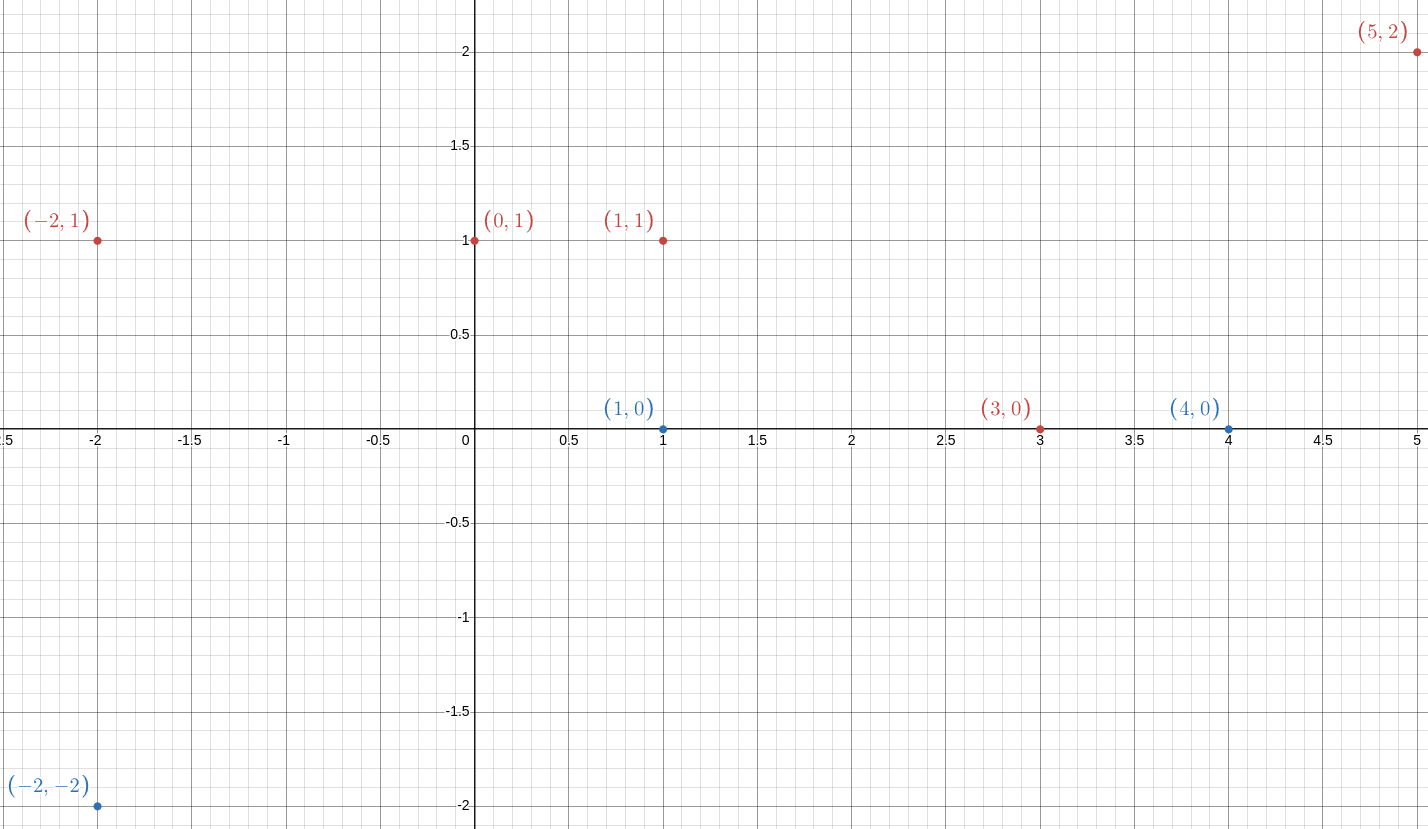
\includegraphics[width=10cm]{img/hw1/data}
            \caption{Blue dots are where $y_i=1$ and red dots are where $y_i=-1$.}
      \end{figure}

      Thus, the perceptron algorithm will never converge no matter how many times we run it over.
}

\subsection{Problem 1b}

\solution{
      We set $w$ to $\vec{0}$ and go through the samples one by one.

      \begin{enumerate}[label=\arabic*:]
            \item $a=0$, which is bad. $w:=w+x_1=\Braket{4, 0}$.
            \item $a=4$, which is bad since $y_2=-1$. $w:=w-x_2=\Braket{3, -1}$.
            \item $a=-1$, OK.
            \item $a=-4$, which is bad since $y_4=1$. $w:=w+x_4=\Braket{1, -3}$.
            \item $a=-5$, OK.
            \item $a=1$, OK.
            \item $a=-1$, OK.
            \item $a=3$, which is bad since $y_8=-1$. $w:=w-x_8=\Braket{-2, -3}$.
      \end{enumerate}
}

\pagebreak

\subsection{Problem 1c}

\solution{
There's four weight vectors that we have:
\begin{itemize}
      \item $w=\Braket{4, 0}$, $c_1=1$
      \item $w=\Braket{3, -1}$, $c_2=2$
      \item $w=\Braket{1, -3}$, $c_3=4$
      \item $w=\Braket{-2, -3}$, $c_4=1$
\end{itemize}
The initial zero vector didn't survive any iterations, so it doesn't matter.

With these parameters, we see that the formula for the perceptron is
\[\sign(\Braket{-2, -3} \cdot x)\]
the formula for the Voted perceptron is
\begin{align*}
        & \sign\left(\sum_{k=1}^{K} c^{(k)} \sign\left(w^{(k)} \cdot x\right)\right) \\
      = & \sign(\sign(\Braket{4, 0} \cdot k)+2\sign(\Braket{3, -1} \cdot k)          \\
        & +4\sign(\Braket{1, -3} \cdot k)+\sign(\Braket{-2, -3} \cdot k))
\end{align*}
and the formula for the Average perceptron is
\[\sign\left(\sum_{k=1}^{K} c^{(k)}w^{(k)} \cdot x\right)=\sign\left(\Braket{-16, -17} \cdot x\right)\]
}

\subsection{Problem 1d}

\solution{
      Here's what each classifier output for each data point:
      \begin{center}
            \begin{tabular}{ |c|c|c|c| }
                  \hline
                  $y$ & Perceptron & Voting & Averaged \\
                  \hline
                  1   & -1         & 1      & -1       \\
                  -1  & -1         & -1      & -1       \\
                  -1  & -1         & -1      & -1       \\
                  1   & 1          & 1      & 1        \\
                  -1  & 1          & -1      & 1        \\
                  1   & -1         & 1      & -1       \\
                  -1  & -1         & -1      & -1       \\
                  -1  & -1         & 1      & -1       \\
                  \hline
            \end{tabular}
      \end{center}
      We see that the accuracies for the three classifiers are 62.5\%, 87,5\%, and 62.5\% respectively.

}

\pagebreak

\section{Problem 2}

\subsection{Problem 2a}

\solution{
      \begin{align*}
            2h_{w'}(x) - 1
             & = \frac{2}{1+e^{-2w^Tx}} - 1                                 \\
             & = \frac{2}{1+e^{-2w^Tx}} - \frac{1+e^{-2w^Tx}}{1+e^{-2w^Tx}} \\
             & = \frac{1-e^{-2w^Tx}}{1+e^{-2w^Tx}}                          \\
             & = \frac{e^{2w^Tx}-1}{e^{2w^Tx}+1}                            \\
             & = \tanh_w(x) \quad\square
      \end{align*}
}

\subsection{Problem 2b}

\solution{
      As $w^Tx \to \infty$, the numerator and denominator become basically the same, so $\tanh_w(x) \to 1$.

      OTOH, as $w^Tx \to -\infty$, the exponential parts go to $0$, so $\tanh_w(x) \to -1$.

      \begin{figure}[h]
            \centering

            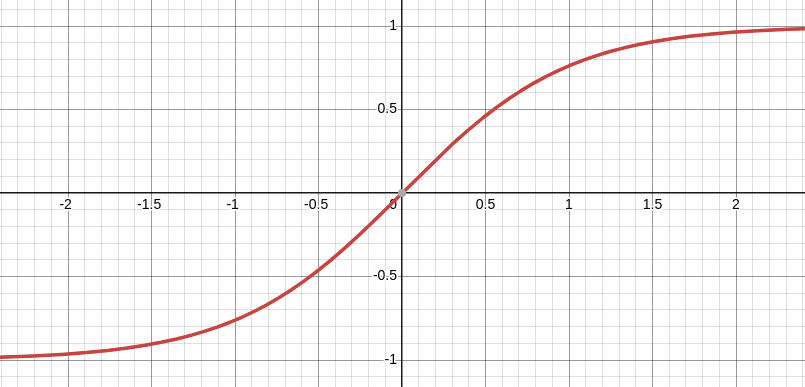
\includegraphics[width=10cm]{img/hw1/tanh}

            \caption{A graph of $\tanh$. $w^Tx$ is the quantity on the $x$-axis.}
      \end{figure}
      As we can see, the middle of the range is exactly $0$, so we can use that as our decision criterion.
}

\subsection{Problem 2c}

\solution{
      As $\tanh$ can give negative values, we can't directly plug it into P2.1
      because $\log$ is undefined for all nonpositives.
}

\subsection{Problem 2d}

\solution{
      The terms in the summation are independent of each other,
      so I'll casework on whether $y_i$ is "yes" or "no" and show that
      the terms in the summation reach their minimum at the same $w$.

      If $y_i$ is positive, then $\tilde{y_i} = y_i = 1$ and the right addend in both
      expressions becomes $0$.

      Simplifying the left addend in P2.2 gets us
      \begin{align*}
            \frac{1+\tilde{y_i}}{2}\log\left(\frac{1+\tanh_w(x_i)}{2}\right)
             & = \log\left(\frac{1+\tanh_w(x_i)}{2}\right)   \\
             & = \log\left(\frac{1+2h_{2w}(x_i)-1}{2}\right) \\
             & = \log(h_{2w}(x_i))
      \end{align*}

      OTOH, if $y_i$ is negative, then the \textit{left} addend becomes $0$.
      Simplifying the right addend gets us
      \begin{align*}
            \frac{1-\tilde{y_i}}{2}\log\left(\frac{1-\tanh_w(x_i)}{2}\right)
             & = \log\left(\frac{1-\tanh_w(x_i)}{2}\right)   \\
             & = \log\left(\frac{1-2h_{2w}(x_i)+1}{2}\right) \\
             & = \log(1-h_{2w}(x_i))
      \end{align*}

      In both cases, we see that we can transform an optimal solution in P2.1
      to an optimal solution in P2.2 by halving all the weights
      and vice versa by doubling all the weights. $\square$
}

\subsection{Problem 2e}

\solution{
      If $\tilde{y_i}=1$, we just need to differentiate the left addend:
      \begin{align*}
            -\frac{\partial}{\partial w} \frac{1+\tilde{y_i}}{2}\log\left(\frac{1+\tanh_w(x_i)}{2}\right)
             & = -\frac{\partial}{\partial w} \log\left(\frac{1+\tanh_w(x_i)}{2}\right)                     \\
             & = -\frac{2}{\log(1+\tanh_w(x_i))} \cdot \frac{1+\frac{\partial}{\partial w} \tanh_w(x_i)}{2} \\
             & = -\frac{1+\frac{4xe^{2w^Tx}}{\left(e^{2w^Tx}+1\right)^2}}{\log(1+\tanh_w(x_i))}
      \end{align*}

      And we do something similar on the right addend for $\tilde{y_i}=-1$:
      \begin{align*}
            -\frac{\partial}{\partial w} \frac{1-\tilde{y_i}}{2}\log\left(\frac{1-\tanh_w(x_i)}{2}\right)
             & = -\frac{\partial}{\partial w} \log\left(\frac{1-\tanh_w(x_i)}{2}\right)                     \\
             & = -\frac{2}{\log(1-\tanh_w(x_i))} \cdot \frac{1-\frac{\partial}{\partial w} \tanh_w(x_i)}{2} \\
             & = -\frac{1-\frac{4xe^{2w^Tx}}{\left(e^{2w^Tx}+1\right)^2}}{\log(1-\tanh_w(x_i))}
      \end{align*}
}

\pagebreak

\section{Problem 3}

\subsection{Problem 3a}

\solution{
      I'll write the $n$th instance as $x_n$ for convenience.

      Again, since the summation's terms are pairwise independent,
      we can just calculate the derivatives on a single term:
      \begin{align*}
            \frac{\partial}{\partial w_0} \alpha_n(w_0+w_1x_n-y_n)^2
             & = \alpha_n \cdot 2(w_0+w_1x_n-y_n) \cdot \frac{\partial}{\partial w_0} w_0    \\
             & = 2\alpha_n(w_0+w_1x_n-y_n)                                                   \\ \\
            \frac{\partial}{\partial w_1} \alpha_n(w_0+w_1x_n-y_n)^2
             & = \alpha_n \cdot 2(w_0+w_1x_n-y_n) \cdot \frac{\partial}{\partial w_1} w_1x_n \\
             & = 2\alpha_n x_n(w_0+w_1x_n-y_n)
      \end{align*}

      With these, we have
      \begin{gather*}
            \frac{\partial J}{\partial w_0} = \boxed{2\sum_{n=1}^{N} \alpha_n(w_0+w_1x_n-y_n)} \\
            \frac{\partial J}{\partial w_1} = \boxed{2\sum_{n=1}^{N} \alpha_n x_n(w_0+w_1x_n-y_n)}
      \end{gather*}
}

\subsection{Problem 3b}

\solution{
      It STP $J(w_0, w_1)$ is convex.

      The Hessian of the function is
      \[\begin{bmatrix}
                  2\sum_{n=1}^{N} \alpha_n     & 2\sum_{n=1}^{N} \alpha_n x_n   \\
                  2\sum_{n=1}^{N} \alpha_n x_n & 2\sum_{n=1}^{N} \alpha_n x_n^2
            \end{bmatrix} = 2\sum_{i=1}^{N} \alpha_n \begin{bmatrix}
                  1   & x_n   \\
                  x_n & x_n^2
            \end{bmatrix}\]

      A positive summation of PSD matrices is still PSD, so we just need to show the PSD-ness of
      \[A=\begin{bmatrix}
                  1   & x_n   \\
                  x_n & x_n^2
            \end{bmatrix}\]

      For any $z=\Braket{a, b}$, we have
      \begin{align*}
            z^TAz
             & = \begin{bmatrix}a+bx_n & ax_n+bx_n^2\end{bmatrix}\begin{bmatrix}a \\ b\end{bmatrix} \\
             & = a^2+2abx_n+bx_n^2                                                                  \\
             & = (a+bx_n)^2                                                                         \\
             & \ge 0\quad\square
      \end{align*}
}

\end{document}
